\chapter{Specifik notsättning för Kårspexet}
\section{Sektioner och repetionsmarkörer}
För att underlätta navigering i noterna på orkesterrep används två sorters markörer. Dessa är \textit{repetitionsmarkörer} och \textit{dubbla taktstreck}. 

Repetitionsmarkörer består av ett eller ett fåtal korta ord i en rektangel som placeras ovanför notraden med vänsterkanten rakt ovanför det taktstreck där en ny sektion börjar. Rep-markörer ska vara korta och koncisa, men bör också vara unika inom ett stycke (det bör inte förekomma samma markör två gånger i en låt). Markörens text ska kunna förstås av både orkester och sångare, vilket betyder att \textit{enskilda bokstäver ej är lämpliga}. Passande namn är istället beskrivningar av vilket sektion av låten man befinner sig i, exempelvis \textbf{VERS 1}, \textbf{INTRO} och \textbf{REFR. 3}.

Dubbla taktstreck används också för att markera sektioner, och alla repetitionsmarkörer måste också ha ett dubbelt taktstreck. Däremot kan dubbla taktstreck utan rep-markör förekomma, exempelvis för att markera halvvägs-punkten i en refräng, eller dela upp ett instrument-break i flera delar. Ett lagom intervall mellan två dubbla taktstreck är generellt mellan 8 och 16 takter, men kan vara så lågt som 2.

Tänk på att om sektionen har en pickup, det vill säga refrängtexten börjar i slutet av sista takten innan refrängen, så ska repetitionsmarkören och det dubbla taktstrecket sitta i början av den första riktiga takten i refrängen, vilket kan bli nästan en hel takt efter att sången påbörjar refrängen.

Formattering för repetitionsmarkörer är färdiginställt i mallen för arrangörer. Använd Musescores inbyggda repetitionsmarkörer med den formattering som medföljer. Av nedanstående exempel är endast den vänstraste korrekt. 

\begin{center}
    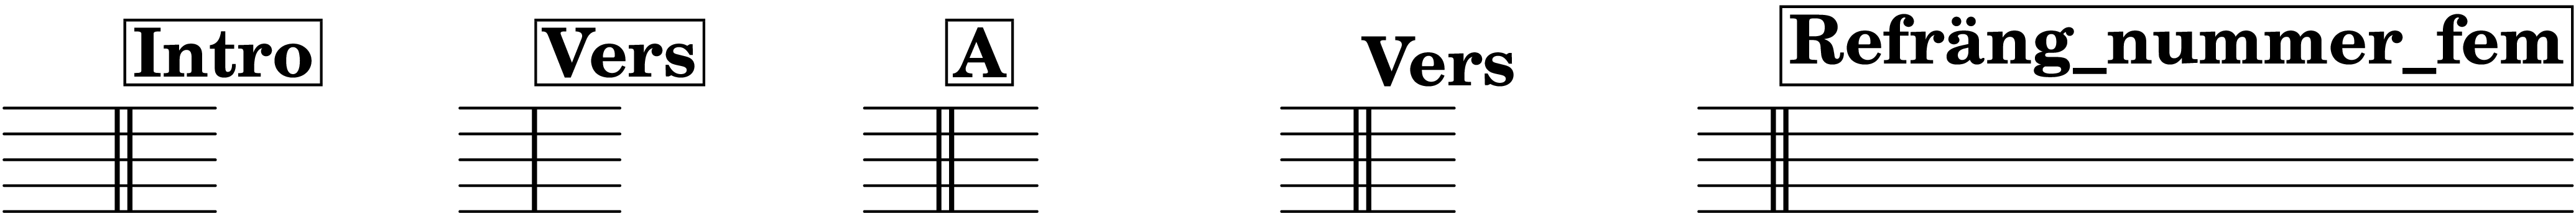
\includegraphics{lilypond/repetition.cropped.png}
\end{center}

\newpage
\section{Papper och partitur}
I mallen för arrangörer är skalning och pappersstorlekar färdiginställda. Partituret använder A3 med 1.55 mm mellan notlinjer, instrumentstämmor A4 med 1.75 mm mellan notlinjer. 

I mallen är även partiturordningen bestämd. Ordningen och grupperingen ska hållas konstant och bör inte ändras. Den är som följer:
\begin{itemize}
    \item Systeminformation (tempoädringar, repetitionsmarkeringar, systemtext etc.)
    \item Träblåsinstrument, i ordningen Flöjt, Oboe, Klarinett, Saxofon, Fagott. \footnote{\label{inom}Inom instrumentgrupperna ordnas instrumenten efter tonhöjd, alltså Sopransaxofon, Altsaxofon, Tenorsaxofon etc. Finns två likadana instrument ordnas de i spelarordning, alltså Flöjt 1, Flöjt 2 etc.}
    \item Bleckblåsinstrument, i ordningen Valthorn, Trumpet, Trombon, Tuba. \footnotemark[\getrefnumber{inom}]
    \item Stråkinstrument, i ordningen Violin, Viola, Cello, Kontrabas. \footnotemark[\getrefnumber{inom}]
    \item Systeminformation (tempoädringar, repetitionsmarkeringar, systemtext etc.)
    \item Skådis.
    \item Trumset, och eventuellt annat slagverk.
    \item Keyboards.
    \item Elgitarr och Elbas.
\end{itemize}

Vissa medlemmar i orkestern kan spela flera instrument. Dessa är markerade \textit{Instrument (Namn)}, exempelvis \textit{Blockflöjt (Alfred)} och längre ned i partituret \textit{Keyboard 2 (Alfred)}. I regel bör bara ett av dessa instrument användas inom en låt, och då två eller fler används tätt inpå varandra ska gott om tid ges att byta instrument. Skriv helt enkelt relevant stämma i det instrument som spelas just då, och lämna andra instrument tomma. \textbf{Ta inte bort överflödiga instrument. Använd inte heller Musescores egen \textit{Change Instrument}-funktion}, då detta skapar problem med stämnamn som försvårar längre fram. Om tomma instrument är en distraktion kan de gömmas i Layout-menyn.

\newpage
\section{Skådis och sång}
Musiken i Kårspexet består ju inte bara av en orkester, utan även av skådespelare som sjunger. Skådis använder sällan noter för att lära sig låtarna, och läser därför oftast inte något ur partituret eller stämmor. Däremot är text och melodi ett ovärderligt navigationsverktyg för mellan skådis, sångchef, kapellmästare och orkester. I partituret bör därför sångmelodi och text stå med. 

Vid den tiden då arrangemanget produceras av arrangören finns troligtvis ingen text skriven. Melodin bör dock ändå finnas med, så som den sjungs i originalet, eller enligt överenskommen låtspecifikation. Text och vem det är som sjunger läggs till senare, av arrangören eller någon annan.

Vem som sjunger markeras i partituret med text ovanför notraden enligt följande:
\begin{enumerate}
    \item Om en enskild skådespelar sjunger noteras karaktärens namn i versaler, exempelvis ``H.C.'' eller ``JENNY''
    \item Om två skådespelare sjunger samma sak (oavsett oktav) markeras detta med ``CHARLES \& KATE''.
    \item Om tre eller fler skådespelare sjunger samma sak (oavsett oktav) markeras detta med ``KATE, JENNY, VICTORIA``.
    \item Om alla skådespelare som är med i numret sjunger samma sak (oavsett oktav) markeras detta med ``ALLA''. Saknas en eller två kan man filtera med ``ALLA utom H.C.'' eller ``ALLA utom OTTO \& JENNY''
    \item Om någon eller några just har sjungit, och alla andra ska sjunga markeras detta med ``ALLA ANDRA''. Detta går att kombinera med tidigare punkter, till exempel ``ALLA ANDRA utom H.C.'' eller ``ALLA ANDRA \& JENNY''.
    \item Om två eller fler skådespelare sjunger homofona stämmor (det vill säga samma rytm och text\footnote{Om texten skiljer sig mellan stämmorna i ett eller ett fåtal ord, exempelvis ``jag'' och ``du'' sätts lättast ett snedstreck mellan orden så att ordningen från vänster till höger stämmer överens med ordningen stämmorna listas uppifrån och ned.} men olika toner) ska stämmorna skrivas på samma notrad och markeras på samma sätt som ovan, men på två eller fler rader, där varje rad korresponderar mot en stämma, ordnade efter tonhöjd i noten. Exempelvis:
\begin{center}
    \begin{tabular}{l}
JENNY \\
ALLA ANDRA utom H.C.
\end{tabular}
\end{center}

    \item Om två eller fler skådespelare sjunger polyfona stämmor, som inte går att notera på en rad, kan en, eller i extremfall fler, extra rad användas. Denna rad ska endast vara synlig just där den behövs, och noterna ska återgå till en rad så fort som möjligt. 

\item Om någon talar en eller ett fåtal meningar samtidigt som musiken spelas markeras detta som följande: 
\begin{center}
    \begin{tabular}{l}
CHARLES \\
"Jo men, han ska ju \\
säkert snart gå."
\end{tabular}
\end{center}
\end{enumerate}

Markeringen är vänsterjusterad, med vänsterkanten rakt ovanför den punkt i musiken där repliken börjar. Repliken ska också ta upp ungefär lika mycket plats horisontellt som den tid det tar att säga repliken. Därför kan det bli många radbrytningar med få ord på varje rad. Detta är inget problem, huvudsaken är inte att det ska vara lätt att läsa innantill, utan att informationen på pappret ska vara så korrekt som möjligt.
